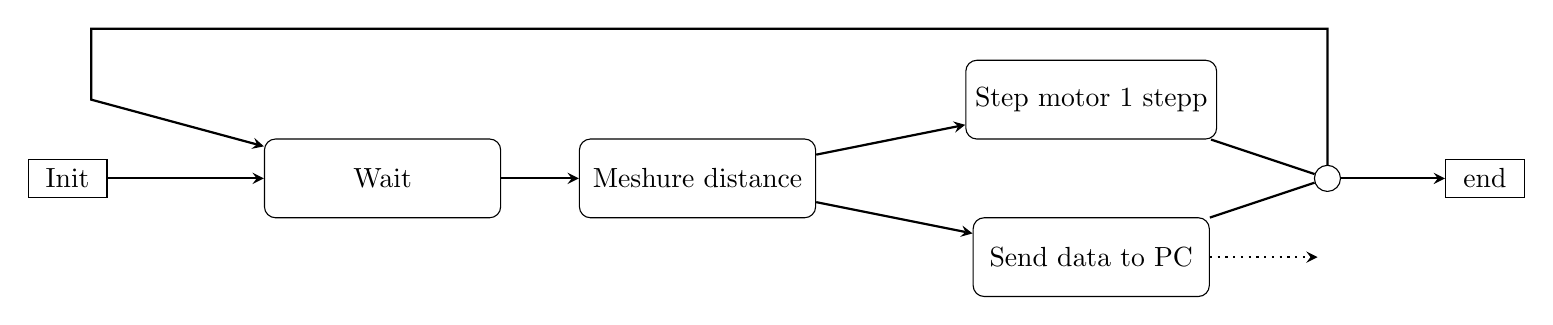
\begin{tikzpicture}
\tikzstyle{startstop} = [rectangle, rounded corners , minimum width=3cm, minimum height=1cm,text centered, draw=black]
\tikzstyle{round}=[circle, minimum width=0cm,draw=black]
\tikzstyle{first} = [rectangle, minimum width=1cm, draw=black]
\tikzstyle{empty}=[]

\usetikzlibrary{shapes.geometric, arrows}
\tikzstyle{arrow} = [thick,->,>=stealth]
\tikzstyle{dottarrow} = [thick, dotted,->,>=stealth]
\tikzstyle{noarrow}=[thick,-=,=stealth]

%nodes
\node (init) [first] {Init};
\node (wait) [startstop, right of =init, xshift=3cm] {Wait};
\node (mesh) [startstop, right of=wait, xshift=3cm] {Meshure distance};
\node (step) [startstop, right of=mesh, xshift=4cm ,yshift=1cm] {Step motor 1 stepp};
\node (send) [startstop, below of=step, yshift=-1cm]{Send data to PC};
\node (merge) [round, right of=send, yshift=1cm, xshift=2cm]{};
\node (end) [first, right of=merge, xshift=1cm] {end};
\node (topc) [empty, right of=send, xshift=2cm]{};

%arrows
\draw [arrow] (wait) -- (mesh);
\draw [arrow] (init) -- (wait);
\draw [arrow] (mesh) -- (step);
\draw [arrow] (mesh) -- (send);
\draw [noarrow] (send) -- (merge);
\draw [noarrow] (step) -- (merge);
\draw [dottarrow] (send) -- (topc);
\draw [arrow] (merge)  -- +(0,1.9)  -- (0.3,1.9) -- (0.3,1) -- (wait);
\draw [arrow] (merge) -- (end);
\end{tikzpicture}